\documentclass[11pt]{article} % use larger type; default would be 10pt

\usepackage{tikz}
\usepackage{pgfplots}
\usetikzlibrary{calc}
\usetikzlibrary{arrows.meta}
\usetikzlibrary{patterns}
        \newcommand\degree[0]{^{\circ}}
\usetikzlibrary{shapes.misc}

\title{Play with TikZ}
\author{Just Us}
%\date{} % Activate to display a given date or no date (if empty),
         % otherwise the current date is printed 

\begin{document}
\pagenumbering{gobble}

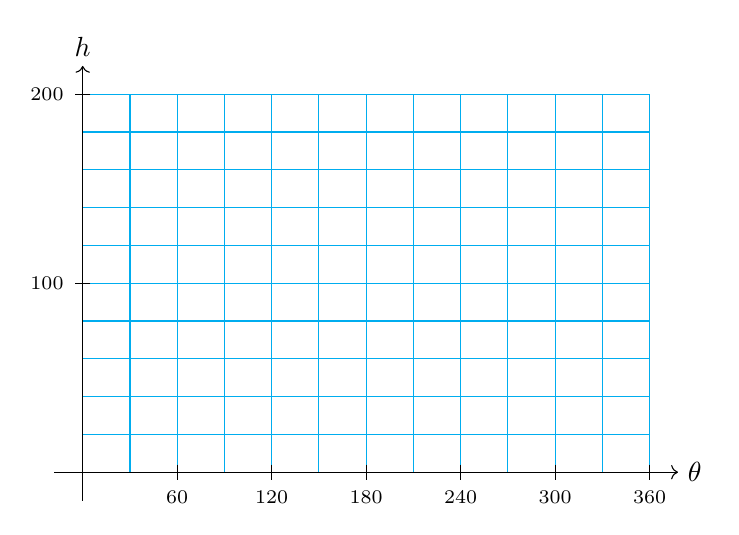
\begin{tikzpicture} [scale=1.2]
\draw[cyan,xstep=0.5,ystep=0.4]
(0,0) grid (6,4);

\draw[->] (-.3,0) -- (6.3,0) node[right] {$\theta$};
\draw[->] (0,-.3) -- (0,4.3) node[above] {$h$};

\foreach \x [evaluate=\x as \xi using int( 60* \x )] in {1,2,...,6}
\draw[black] ($ \x *(1,0) +(0,.08) $) --++(0,-.16) node[anchor=north, xshift=0,yshift=-3, fill=white, inner sep=1pt] {\scriptsize$ \xi $};

\foreach \y  [evaluate=\y as \yi using int( 50* \y )] in {2,4}
\draw[black] (.08,\y ) --++(-.16,0) node[anchor=east, xshift=-3, fill=white, inner sep=1pt] {\scriptsize\yi};

\end{tikzpicture}





\end{document}
